\begin{surferPage}[D5+- Singularity]{$D_5^{+-}$ Singularity}
Visually, the $D_5^{+-}$ singularity is certainly one of the most appealing simple singularities of all.
It looks like a rock with an apex dancing on top of a smooth mountain right at the most fragile point
of a thin passage from one part of the mountain to another.

    \begin{center}
        \begin{tabular}{@{}c@{}}
          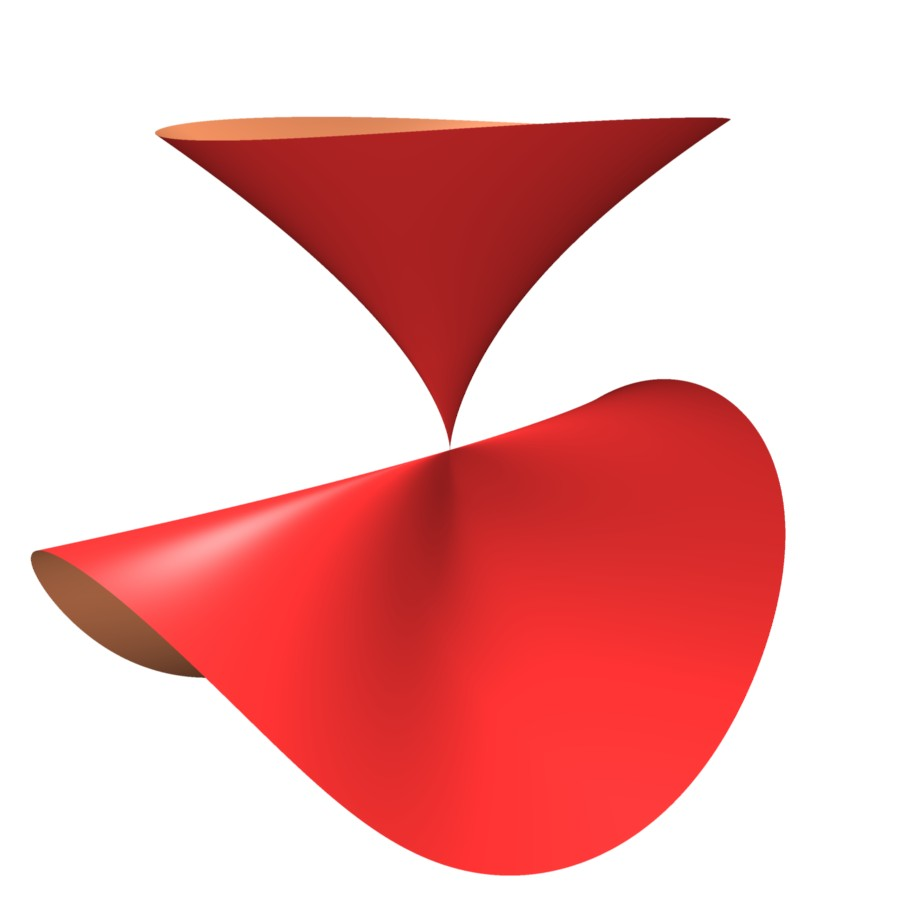
\includegraphics[width=1.1cm]{../../common/images/D5pm}
        \end{tabular}
    \end{center}
    \vspace*{-0.4em}
        \vspace*{-0.4em}
    \begin{center}
      $x^2y+y^4-z^2=0.$
    \end{center}
    \vspace*{-0.4em}


The $D_4$ singularity has a $y^3$ at the place of the equation where the $D_5$ has a $y^4$,
so we can easily deform the $D_5$ into a $D_4$ singularity and vice versa.
In this way, it is possible to experience how the $D_5$ develops from the $D_4$ by shrinking
the lower whole until it is gone.

    \begin{center}
      \begin{tabular}{@{}c@{\quad}c@{\quad}c@{}}
        \begin{tabular}{@{}c@{}}
          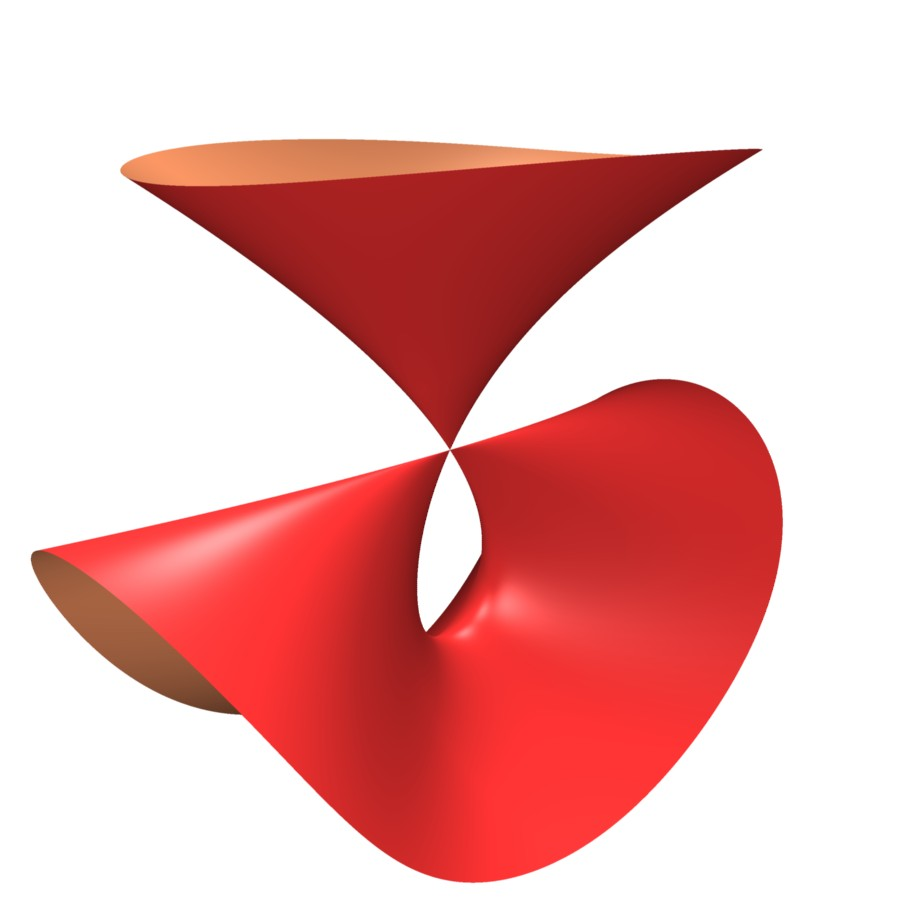
\includegraphics[width=1.1cm]{../../common/images/D5pm_03}
        \end{tabular}
        &
        \begin{tabular}{@{}c@{}}
          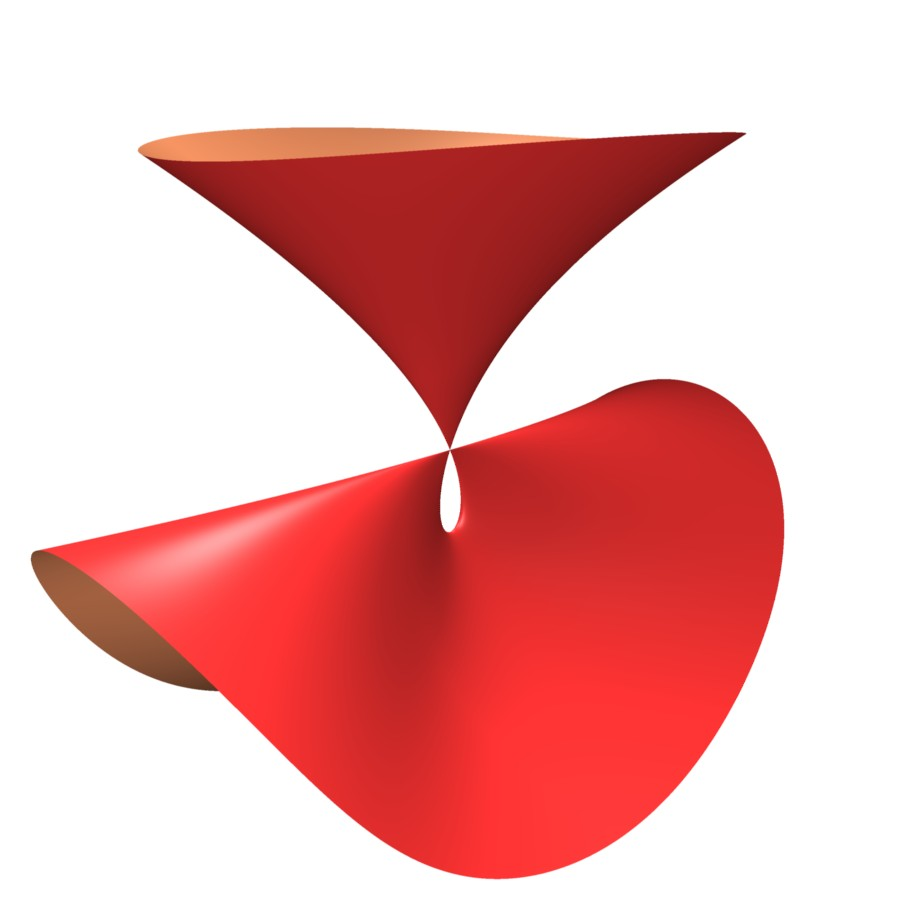
\includegraphics[width=1.1cm]{../../common/images/D5pm_02}
        \end{tabular}
        &
        \begin{tabular}{@{}c@{}}
          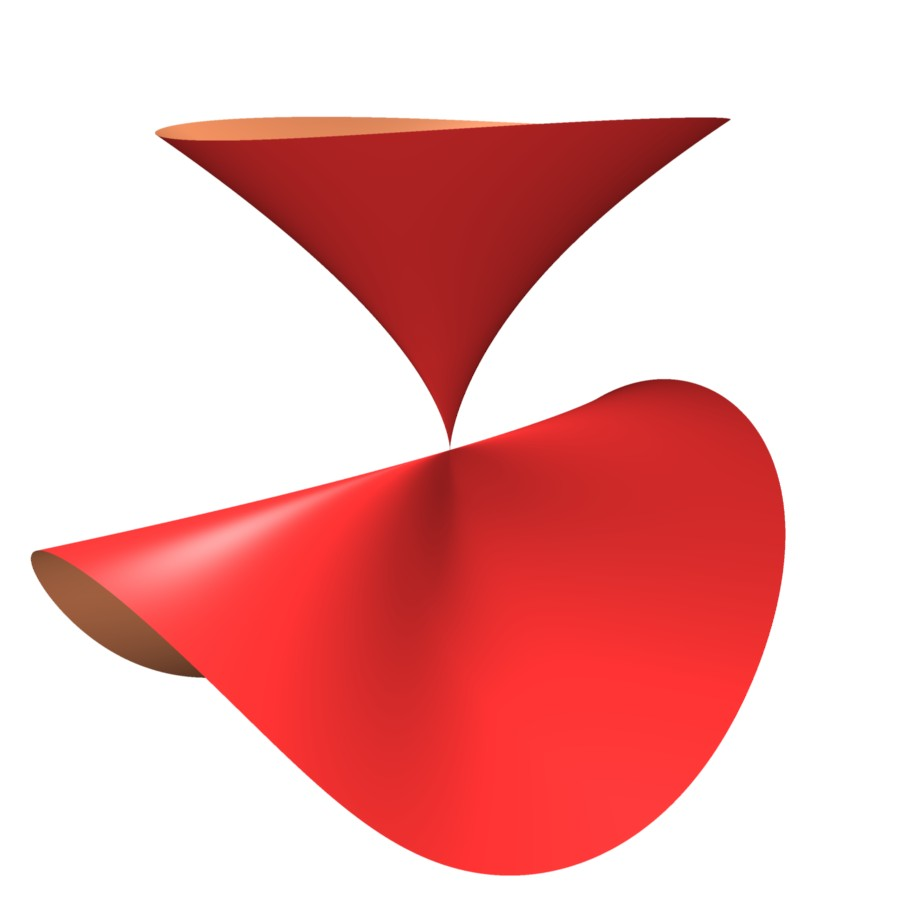
\includegraphics[width=1.1cm]{../../common/images/D5pm_01}
        \end{tabular}
      \end{tabular}
    \end{center}
    \vspace*{-0.4em}

Alternatively, one can move the mountain up while keeping the position of the apex of the rock.
This causes the rock to split into a real (visible) and an imaginary (invisible) part.

    \begin{center}
      \begin{tabular}{@{}c@{\quad}c@{\quad}c@{}}
        \begin{tabular}{@{}c@{}}
          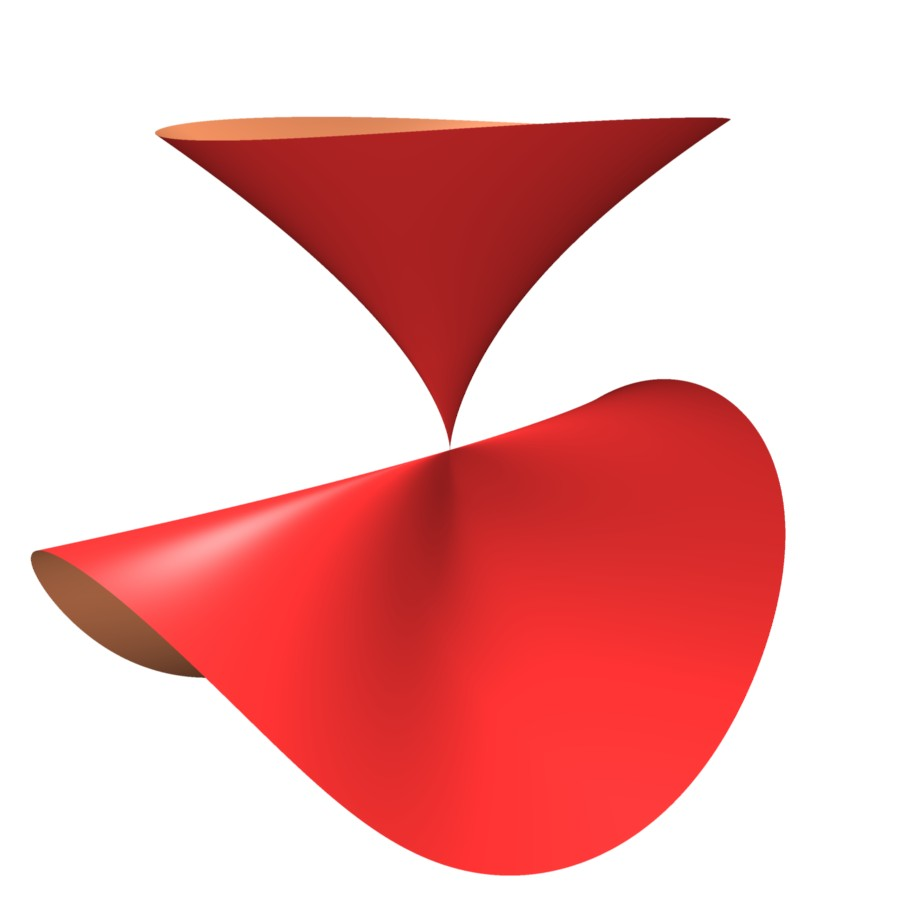
\includegraphics[width=1.1cm]{../../common/images/D5pm_01}
        \end{tabular}
        &
        \begin{tabular}{@{}c@{}}
          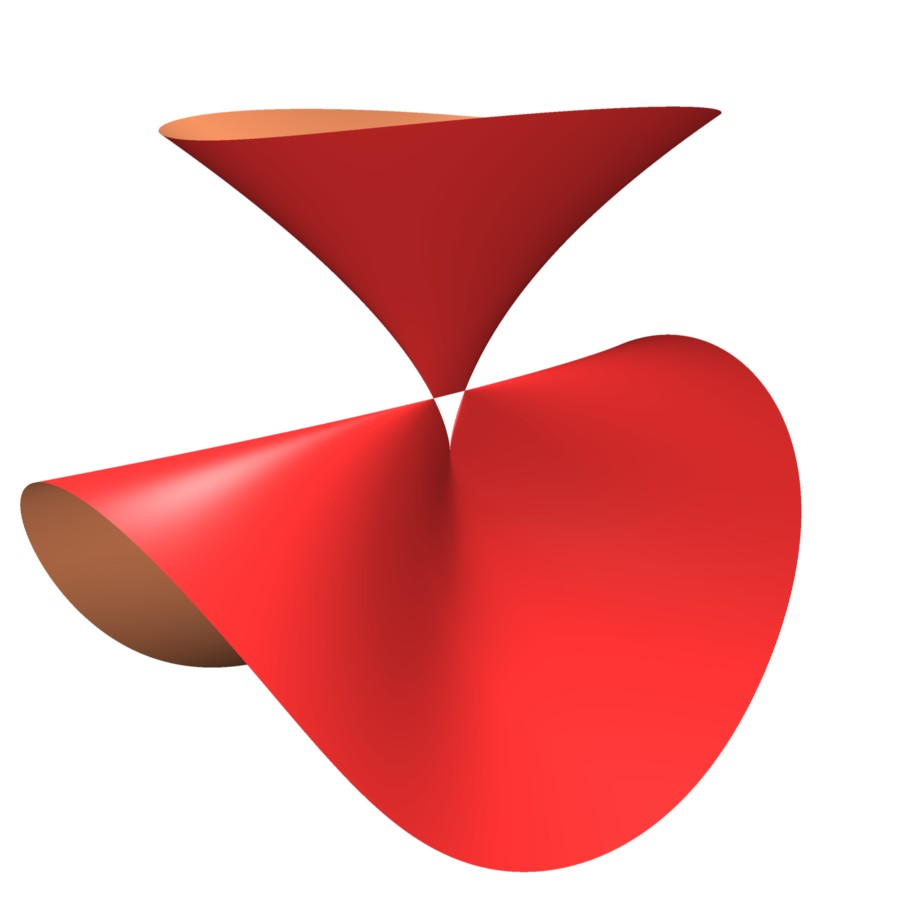
\includegraphics[width=1.1cm]{../../common/images/D5pm_04}
        \end{tabular}
        &
        \begin{tabular}{@{}c@{}}
          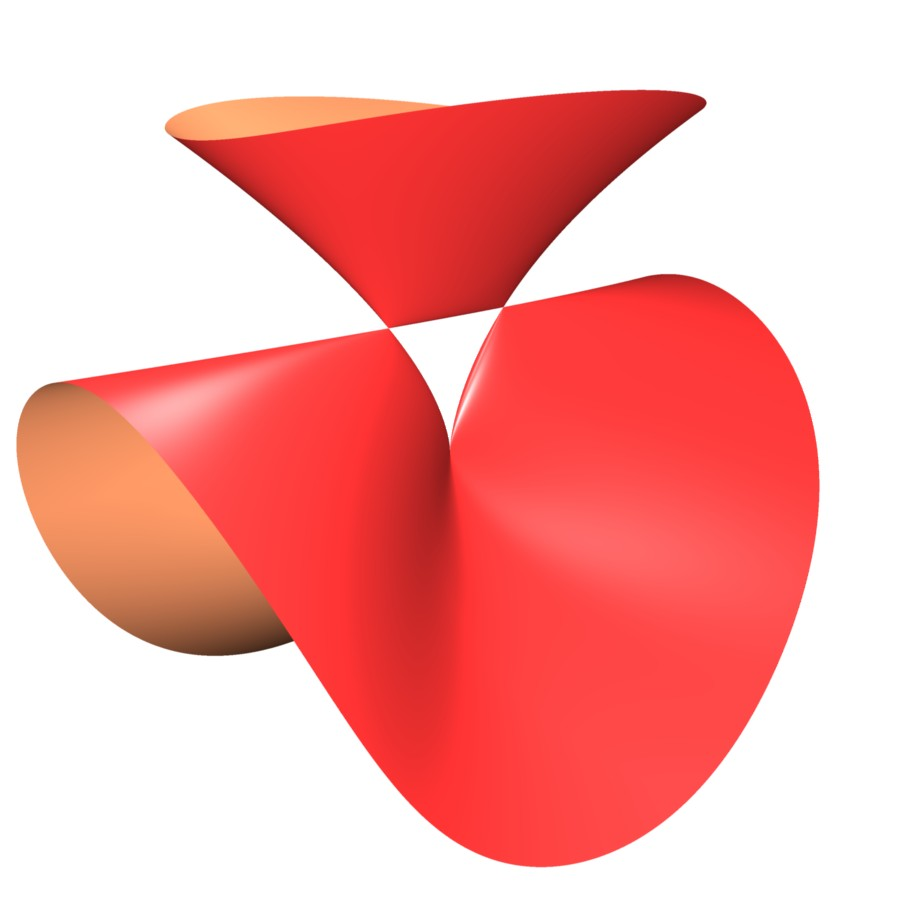
\includegraphics[width=1.1cm]{../../common/images/D5pm_05}
        \end{tabular}
      \end{tabular}
    \end{center}
    \vspace*{-0.4em}

\end{surferPage}
